% Appendix counters are independent of the main text.
\setcounter{figure}{0}
\setcounter{table}{0}
\renewcommand{\thefigure}{A\arabic{figure}}
\renewcommand{\thetable}{A\arabic{table}}
\renewcommand{\theHfigure}{appendix.\arabic{figure}}
\renewcommand{\theHtable}{appendix.\arabic{table}}

\section{Data and evaluation settings}
\label{app:domains}

\subsection{Task scope, resources, and evaluation dimensions}
\label{app:domain-signals}
A domain has a fixed quality standard and a separately adapted evaluator.
Table~\ref{tab:data-sources} lists the 19 equally weighted C1 domains, their resources, Seed criterion sources, and candidate signals.
Rubric judges can supply dimensional and overall judgments.
The executed signal subset is frozen before mining; reference-based metrics require permitted references, and reserved assessment signals remain outside search.

\paragraph{Seed construction and attribution.}
Seed is our domain-specific implementation, not a released evaluator copied from a benchmark.
We adapt published rubric criteria where available and otherwise write criteria from the task requirements and cited evaluation protocols.
The table identifies these sources alongside our additions; borrowing a criterion does not imply reusing its original judge prompt, model, or score scale.
We assemble the prompts, tool routing, and score aggregation, freezing one initial checkpoint per domain before comparative search, without Val/Test preference feedback.
All optimizers receive that checkpoint, subject to their declared editable spaces (Table~\ref{tab:adaptation}).

\begingroup
\small
\setlength{\tabcolsep}{4pt}
\renewcommand{\arraystretch}{1.08}
\begin{longtable}{@{}P{3.45cm}P{3.55cm}P{5.68cm}@{}}
\caption{Task scope, data resources, Seed criterion sources, and candidate signals across the 19 domains. Numbers link methods to dimensions within each row. Sources inform criteria or checks; listed signals are not all required Seed components.}
\label{tab:data-sources}\\
\toprule
Domain, task and data sources & Seed criteria and sources & Corresponding methods and signals\\
\midrule
\endfirsthead
\multicolumn{3}{l}{\small Table~\thetable\ continued}\\
\toprule
Domain, task and data sources & Seed criteria and sources & Corresponding methods and signals\\
\midrule
\endhead
\bottomrule
\endfoot
\multicolumn{3}{l}{\textit{Structured visual artifacts}}\\*
\textbf{TD-SV1} Brief-conditioned single-slide generation\newline Our human-annotated slide comparisons & (1) Brief adherence; (2) content correctness; (3) readability; (4) visual hierarchy; (5) layout consistency\newline\emph{Our brief/content rubric; visual checks informed by SlideAudit \citep{zhang2025slideaudit}.} & (1--2) Brief-to-text coverage and factuality checks; (3) font-size and contrast diagnostics; (4--5) PPTX/render geometry, overlap and alignment checks, supplemented by visual rubric judgments.\\
\addlinespace
\textbf{TD-SV2} Screenshot-conditioned webpage reconstruction\newline \href{https://huggingface.co/datasets/SALT-NLP/Design2Code}{Design2Code}; \href{https://huggingface.co/datasets/SALT-NLP/Design2Code_human_eval_pairwise}{human-pair release} & (1) Text fidelity; (2) position and structure; (3) color and style; (4) visual detail\newline\emph{Adapted from Design2Code's reconstruction metrics; visual detail added.} & (1--3) Design2Code text, position, color and block-match scores \citep{si2025design2code}; (4) screenshot SSIM \citep{wang2004ssim} and CLIP/DINO similarity \citep{radford2021clip,caron2021dino} as visual proxies.\\
\addlinespace
\textbf{TD-SV3} Specification-conditioned webpage generation\newline \href{https://huggingface.co/datasets/lmarena-ai/webdev-arena-preference-10k}{WebDev Arena}; \href{https://huggingface.co/datasets/luzimu/WebGen-Bench}{WebGen-Bench} \citep{lu2025webgen} & (1) Requirement fulfillment; (2) functionality; (3) usability; (4) visual quality\newline\emph{Adapted from WebGen-Bench's functionality and visual evaluation; usability added.} & (1--2) Browser interaction and requirement checklists; (3) \href{https://github.com/dequelabs/axe-core}{axe-core} accessibility checks; (4) \href{https://huggingface.co/datasets/luzimu/WebGen-Bench}{WebGen-Bench} visual evaluation.\\
\addlinespace
\textbf{TD-SV4} Source-grounded slide-deck generation\newline \href{https://huggingface.co/datasets/PresentBench/PresentBench}{PresentBench}; PPTAgent \citep{pptagent2025} & (1) Source fidelity and coverage; (2) organization; (3) visual consistency and readability; (4) editability\newline\emph{PresentBench content checklists and PPTAgent/SlidesGen-Bench quality criteria.} & (1) PresentBench checklists \citep{presentbench2026}; (2) deck-level organization and repetition checks; (3--4) \href{https://github.com/yunqiaoyang/SlidesGen-Bench}{SlidesGen-Bench} \citep{yang2026slidesgen} aesthetics/editability protocols and PPTX diagnostics.\\
\addlinespace
\textbf{TD-SV5} Topic-conditioned slide-deck generation\newline \href{https://huggingface.co/datasets/Yqy6/Slides-Align}{Slides-Align} \citep{yang2026slidesgen}; \href{https://github.com/yunqiaoyang/SlidesGen-Bench}{SlidesGen-Bench} & (1) Topic relevance and correctness; (2) narrative organization; (3) aesthetics and readability; (4) cross-page consistency\newline\emph{SlidesGen-Bench visual criteria; topic correctness and organization added.} & (1--2) Deck-level rubric judgments; (3) \href{https://github.com/yunqiaoyang/SlidesGen-Bench}{SlidesGen-Bench} aesthetics protocol; (4) cross-page typography, palette and layout checks.\\
\addlinespace
\multicolumn{3}{l}{\textit{Image generation and understanding}}\\*
\textbf{TD-IG1} Detailed image-caption generation\newline \href{https://github.com/njucckevin/CapArena}{CapArena} \citep{cheng2025caparena}; DOCCI \citep{onoe2025docci} & (1) Factuality and relations; (2) content coverage; (3) detail; (4) conciseness and organization\newline\emph{Adapted from CapArena's precision, informativeness, hallucination, and conciseness guidance.} & (1,3) Atomic visual-claim checks; (2) reference-based CIDEr/SPICE \citep{vedantam2015cider,anderson2016spice}; (4) rubric judgments. \href{https://github.com/jmhessel/clipscore}{CLIPScore} \citep{hessel2021clipscore} supplies a complementary image--text alignment signal.\\
\addlinespace
\textbf{TD-IG2} Text-to-image generation\newline \href{https://huggingface.co/datasets/ymhao/HPDv2}{HPDv2} \citep{wu2023hpsv2}; \href{https://huggingface.co/datasets/zai-org/ImageRewardDB}{ImageRewardDB} & (1) Prompt alignment; (2) compositional relations; (3) visual quality; (4) overall preference\newline\emph{Our rubric combines ImageReward/HPDv2 preference criteria with compositional checks.} & (1) CLIP similarity; (1--2) \href{https://arxiv.org/abs/2303.11897}{TIFA} \citep{hu2023tifa}/\href{https://arxiv.org/abs/2310.18235}{DSG} \citep{cho2024dsg} visual questions, GenEval checks \citep{ghosh2023geneval}; (3) visual rubric judgments; (4) PickScore \citep{kirstain2023pickapic}, ImageReward \citep{xu2023imagereward}, \href{https://github.com/tgxs002/HPSv2}{HPSv2}.\\
\addlinespace
\textbf{TD-IG3} Single-source instruction-based image editing\newline \href{https://huggingface.co/datasets/TIGER-Lab/GenAI-Bench}{GenAI Arena} \citep{jiang2024genaiarena}; \href{https://huggingface.co/datasets/osunlp/MagicBrush}{MagicBrush} \citep{zhang2023magicbrush} & (1) Instruction fulfillment; (2) content preservation; (3) edit quality and naturalness\newline\emph{GIE-Bench instruction/preservation checks; our visual-quality rubric.} & (1--2) \href{https://arxiv.org/abs/2505.11493}{GIE-Bench} \citep{qian2025gie} visual questions and preservation checks; (2) masked DINO/LPIPS; (3) visual rubric judgments. \href{https://arxiv.org/abs/2509.26346}{EditReward} \citep{wu2026editreward} supplies a separate preference signal.\\
\addlinespace
\textbf{TD-IG4} LR-conditioned image super-resolution\newline \href{https://huggingface.co/datasets/casyssong/RefSR-18K}{RefSR-18K} \citep{song2026refsr}; \href{https://github.com/yushuaisong/RefReward-SR}{RefReward-SR} & (1) Fidelity; (2) detail and texture; (3) artifacts and naturalness\newline\emph{Our fidelity/quality rubric, informed by RefReward-SR's evaluation setting.} & (1) Reference-based PSNR/SSIM; (2--3) \href{https://github.com/richzhang/PerceptualSimilarity}{LPIPS} \citep{zhang2018lpips} and visual rubric judgments. \href{https://github.com/yushuaisong/RefReward-SR}{RefReward-SR} supplies a separate preference signal.\\
\addlinespace
\textbf{TD-IG5} Text-to-3D object generation\newline \href{https://huggingface.co/datasets/ccccby/MATE-3D}{MATE-3D} \citep{zhang2025mate3d}; \href{https://huggingface.co/datasets/3DGen/3DGen-Bench}{3DGen-Bench} \citep{zhang20253dgen} & (1) Text alignment; (2) geometry and completeness; (3) texture; (4) multiview consistency\newline\emph{T3Bench alignment and multiview quality protocol; our geometry/texture checks.} & (1) \href{https://arxiv.org/abs/2310.02977}{T3Bench} \citep{he2023t3bench} text--3D alignment protocol; (2) mesh diagnostics; (2--4) T3Bench multiview quality evaluation and fixed-view visual rubric judgments.\\
\addlinespace
\textbf{TD-IG6} Image-to-3D object generation\newline \href{https://huggingface.co/datasets/3d-arena/3d-arena}{3D Arena} \citep{ebert20253darena}; 3DGen-Bench & (1) Source-image fidelity; (2) geometry; (3) texture; (4) multiview consistency\newline\emph{Our source-conditioned adaptation of 3D quality checks; 3D Arena supplies comparisons.} & (1) Camera-aligned source-view CLIP/DINO similarity; (2) mesh diagnostics; (3--4) visual rubric judgments across standardized renders.\\
\addlinespace
\multicolumn{3}{l}{\textit{Text generation}}\\*
\textbf{TD-TG1} Source-grounded document summarization\newline \href{https://huggingface.co/datasets/openai/summarize_from_feedback}{summarize-from-feedback} \citep{stiennon2020summarize} & (1) Source faithfulness; (2) coverage; (3) relevance; (4) coherence and conciseness\newline\emph{Adapted from summarization feedback and SummEval criteria \citep{fabbri2021summeval}.} & (1) \href{https://github.com/tingofurro/summac}{SummaCConv} \citep{laban2022summac}; (2--3) reference-based \href{https://github.com/google-research/google-research/tree/master/rouge}{ROUGE} \citep{lin2004rouge}/\href{https://github.com/Tiiiger/bert_score}{BERTScore} \citep{zhang2020bertscore} similarity and source-coverage checks; (4) rubric judgments.\\
\addlinespace
\textbf{TD-TG2} RAG-supported long-form answer generation\newline \href{https://github.com/YuchenFan48/LFQA-E}{LFQA-E} \citep{fan2026lfqae}; \href{https://github.com/princeton-nlp/ALCE}{ALCE} \citep{gao2023alce} & (1) Correctness and coverage; (2) evidence support; (3) citation precision and completeness; (4) clarity\newline\emph{ALCE evidence/citation checks; our answer-quality rubric informed by LFQA-E.} & (1,4) Question-conditioned rubric judgments; (2) claim--evidence entailment; (3) \href{https://github.com/princeton-nlp/ALCE}{ALCE} citation precision/recall.\\
\addlinespace
\textbf{TD-TG3} Machine translation\newline \href{https://github.com/google/wmt-mqm-human-evaluation}{WMT MQM} \citep{freitag2021mqm}; \href{https://huggingface.co/datasets/FinnSchmidt/CD-ESA}{CD-ESA} \citep{schmidt2026cdesa} & (1) Accuracy; (2) fluency; (3) terminology; (4) omissions and additions; (5) style\newline\emph{Adapted from MQM's error taxonomy; omissions/additions made explicit.} & (1--5) MQM-style error judgments; \href{https://github.com/Unbabel/COMET}{COMET} \citep{rei2020comet} supplies aggregate translation quality, with \href{https://github.com/mjpost/sacrebleu}{SacreBLEU/chrF} \citep{post2018sacrebleu,popovic2015chrf} as reference-overlap signals.\\
\addlinespace
\textbf{TD-TG4} Instruction-constraint-following response generation\newline \href{https://github.com/thu-coai/IF-RewardBench}{IF-RewardBench} \citep{wen2026ifreward} & (1) Explicit constraint satisfaction; (2) correctness; (3) usefulness and relevance; (4) expression\newline\emph{IFEval/IF-RewardBench constraint checks; our general response-quality criteria.} & (1) \href{https://arxiv.org/abs/2311.07911}{IFEval} \citep{zhou2023ifeval} strict/loose checks and task-specific constraint checkers; (2--4) rubric judgments, informed by \href{https://github.com/thu-coai/IF-RewardBench}{IF-RewardBench} checklists.\\
\addlinespace
\textbf{TD-TG5} Open-ended dialogue-response generation\newline \href{https://huggingface.co/datasets/nvidia/HelpSteer2}{HelpSteer2} \citep{wang2024helpsteer,wang2025helppref} & (1) Helpfulness; (2) correctness; (3) contextual consistency; (4) relevance and expression; (5) safety\newline\emph{HelpSteer2 helpfulness, correctness, and coherence; relevance/expression adapted, safety added.} & (1--5) Dimensional dialogue rubric judgments; (3) history--response contradiction checks. A compatible public reward model supplies a separate overall signal.\\
\addlinespace
\multicolumn{3}{l}{\textit{Automated research}}\\*
\textbf{TD-AR1} Research-idea generation\newline \href{https://huggingface.co/datasets/yolo1213811/research-ideation-arena-dataset}{Research Ideation Arena} \citep{chen2026ideation} & (1) Novelty; (2) feasibility; (3) significance; (4) specificity\newline\emph{Adapted from Ideation Arena's four expert-review criteria.} & (1--4) Ideation Arena human-review rubric; (1,3) comparison with the supplied literature and claim--source support checks.\\
\addlinespace
\textbf{TD-AR2} ML/NLP ablation-plan generation\newline \href{https://huggingface.co/datasets/yale-nlp/AbGen}{AbGen} \citep{zhao2025abgen} & (1) Importance; (2) faithfulness; (3) soundness, including controls and executability\newline\emph{Adapted from AbGen-Eval's three criteria; controls/executability operationalize soundness.} & (1--3) \href{https://huggingface.co/datasets/yale-nlp/AbGen}{AbGen-Eval} rubric judgments; (2) proposal--paper alignment; (3) intervention/control/outcome checks and confound diagnostics.\\
\addlinespace
\textbf{TD-AR3} Peer-review critique generation\newline \href{https://huggingface.co/datasets/Reza8848/AAAR-1.0}{AAAR} \citep{lou2025aaar}; \href{https://github.com/TU2021/PaperAudit}{PaperAudit} \citep{tu2026paperaudit} & (1) Correctness and evidence; (2) significance and coverage; (3) actionability; (4) fairness and clarity\newline\emph{Our critique-quality rubric; AAAR/PaperAudit inform evidence and error checks.} & (1) Paper-evidence localization and \href{https://github.com/TU2021/PaperAudit}{PaperAudit} error checks on annotated subsets; (2--4) critique-quality rubric judgments.\\
\end{longtable}
\endgroup


SV1 uses our own human-annotated slide comparisons; SlideAudit informs visual criteria rather than supplying these preference labels.
For public resources, human dimensional labels can support criterion-specific evaluation; they are not relabeled as overall preferences.
Cohort construction must match each judgment to its artifacts, criterion, and permitted evidence.
SV5 uses aesthetic ranks, IG5 overall MOS, TG3 segment scores, and AR2 a three-dimension composite; these human-derived orderings are reported separately from direct choices in a sensitivity analysis.
Admission requires a frozen source version, permission for the intended processing, executable inputs, and an independent test cohort.

References, dimensional scores, and metric-training resources do not automatically supply independent overall preferences.
DOCCI supplies caption references \citep{onoe2025docci} and SummEval supplies CNN/DailyMail dimensional ratings, not TL;DR pair labels \citep{fabbri2021summeval}.
Resources used to train a metric require an overlap audit before independent evaluation.

\subsection{Feedback and preference mining}
\label{app:annotation}
Human feedback has four levels: $H_0$ gives overall preferences; $H_1$ gives dimensional preferences; $H_2$ identifies error type, severity, and location; $H_3$ optionally supplies a free-form rationale.
Missing feedback remains absent.
Existing-label replay counts revealed source groups and pairs; new annotation additionally records requested ratings, person-time, abstentions, and adjudication.
Freeze rubrics, permitted evidence, tie rules, rater qualifications, compensation, and review requirements.
Development uses two independent judgments with adjudication, final assessment uses three, and both hide method identities, earlier winners, and model scores while randomizing presentation.

Mining uses deduplicated Train groups under the signal normalization and voting rules in Section~\ref{sec:mining}.
Signal definitions, source groups, dimension mappings, tie margins, and repeats are frozen before label access.
The hash-selected random anchor is independent of scores and counts toward the total label budget.
The four judges in Table~\ref{tab:run-config} form four source groups; repeats, prompt variants, and the Seed's use of the same model do not add groups or establish independent errors.
Within-dimension opposition determines rank, with pair IDs breaking ties.

A model signal uses the median of same-repeat score differences; this differs from comparing each artifact's median final score in Equation~\ref{eq:measurement}.
The native runner uses three repeats and a two-point tie margin for model scores; metric bundles specify their own margins.
A missing required repeat makes a signal unavailable, not an agreement.
Metrics reserved for final assessment are excluded from mining and evaluator tools.
The signal roster and anchor fraction are specified in Table~\ref{tab:run-config}.

\subsection{Data allocation and evaluation protocol}
\label{app:boundaries}
\label{app:measurement}
\label{app:configuration}

\paragraph{Splits and allocations.}
Before mining, split original-input groups and declared dependence groups into Train, Val, and Test without using labels or mining scores.
Keep document derivatives, website templates, related images, and research topics together where applicable.
All methods share the frozen source pool, eligibility rules, and held-out pairs, with no later Val/Test additions or replacements.
Train supplies feedback and traces for revision; Val permits only checkpoint retention, releasing the promotion indicator and retained score to the optimizer.
Test is assessed offline after search and selection rules are frozen.
The deployed scorer sees one output and permitted evidence, not opponents, human labels, generator identity, or split metadata.

Table~\ref{tab:cohort-allocation} counts deduplicated original-input groups, each contributing one C1 pair selected by fixed hash before label inspection.
Tune is included in Train but excluded from preference mining; Feedback counts revealed groups.
Val/Test allocations precede annotation, with decisive pairs, ties, abstentions, and missing assets reported separately.
Source versions, hashes, grouping keys, filters, and pair IDs are recorded in the release manifest.
Insufficient eligible groups require collection or a protocol revision, not extra dependent pairs counted as new inputs.
For the four analysis domains, the public files contain 6,041 single-turn WebDev requests, 3,400 CapArena images with strict preferences, 20,986 TL;DR posts with comparisons, and 1,782 ideation contexts with strict overall preferences.
These are source capacities before grouping and eligibility checks, not final cohorts.
Appendix~\ref{app:downstream} specifies separate C2/C3 inputs and cross-source exclusions.

\begin{table}[!htbp]
\caption{\textbf{C1 data allocation by domain.} Train includes Tune; Feedback is drawn from the remaining Train pool. Every count is in original-input groups. Resource roles and evaluation dimensions are in Table~\ref{tab:data-sources}.}
\label{tab:cohort-allocation}
\centering\small
\setlength{\tabcolsep}{3pt}
\begin{tabularx}{\linewidth}{@{}lYrrrrr@{}}
\toprule
ID & Cohort source & Train & Tune & Feedback & Val & Test\\
\midrule
SV1 & Our human-annotated slide comparisons & 200 & 20 & 100 & 40 & 120\\
SV2 & Design2Code human-pair release & 240 & 32 & 100 & 80 & 160\\
SV3 & WebDev Arena & 256 & 32 & 100 & 64 & 200\\
SV4 & PresentBench; new deck pairs & 120 & 16 & 80 & 40 & 78\\
SV5 & Slides-Align & 90 & 10 & 50 & 30 & 67\\
IG1 & CapArena human comparisons & 256 & 32 & 100 & 64 & 200\\
IG2 & HPDv2 & 256 & 32 & 100 & 64 & 200\\
IG3 & MagicBrush sources; new edited pairs & 128 & 16 & 100 & 32 & 64\\
IG4 & RefSR-18K & 256 & 32 & 100 & 64 & 200\\
IG5 & MATE-3D & 80 & 10 & 50 & 30 & 50\\
IG6 & 3D Arena; new overall judgments & 128 & 16 & 100 & 32 & 64\\
TG1 & Summarize-from-feedback, TL;DR only & 256 & 32 & 100 & 64 & 200\\
TG2 & LFQA-E with fixed evidence bundles & 256 & 32 & 100 & 64 & 200\\
TG3 & WMT MQM; document-level grouping & 256 & 32 & 100 & 64 & 200\\
TG4 & IF-RewardBench & 256 & 32 & 100 & 64 & 200\\
TG5 & HelpSteer2 preference release & 256 & 32 & 100 & 64 & 200\\
AR1 & Research Ideation Arena & 256 & 32 & 100 & 64 & 200\\
AR2 & AbGen-Eval & 50 & 10 & 40 & 20 & 30\\
AR3 & AAAR; new overall judgments & 128 & 16 & 100 & 32 & 64\\
\bottomrule
\end{tabularx}
\end{table}

\paragraph{Experimental allocation and replication.}
Table~\ref{tab:experiment-allocation} specifies data, replication, and allowances.
Four-domain analyses reuse C1 Val/Test groups but run fresh searches for changed feedback or policies; the mining interaction reuses matching 100-group runs without counting them as new replications.
Evaluator search, refinement, and training have separate budgets.

\begin{table}[!htbp]
\caption{\textbf{Allocation across experiments.} The four-domain subset is SV3, IG1, TG1, and AR1. A search cap is 100 units as defined in Table~\ref{tab:run-config}.}
\label{tab:experiment-allocation}
\centering\small
\begin{tabularx}{\linewidth}{@{}P{2.4cm}YP{3.7cm}@{}}
\toprule
Experiment & Data per domain and condition & Replication and allowance\\
\midrule
C1 optimizer comparison & Table~\ref{tab:cohort-allocation}; identical revealed feedback for every optimizer & 5 seeds; 100 units/search\\
Search ablations & Four domains; 100 revealed groups; common 64 Val and 200 Test groups & Full plus 8 controls; 5 seeds; 100 units/search\\
Controller tuning & 32 Tune groups per analysis domain, disjoint from preference mining & $k\in\{2,4,6\}$; 2 seeds; 10 units per setting/seed\\
Mining replay & Four domains; 20/50/100/200 revealed groups from the 224-group sampling pool & Random, uncertainty, cross-model, full; 5 seeds and 100 search units at each budget\\
Anchor and interaction & Four domains; 100 revealed groups; 20\% versus no anchor; random/mined $\times$ fixed-patience/EvalOpt & 5 seeds; common search cap; reuse matching cells\\
Controlled diagnostics & Four domains; 20 Train-derived instances per failure type; 3 types & 5 seeds; at most 6 attempts and 10 units per instance\\
Natural trajectories & 30 directions/domain from the full-method searches, stratified by confirmation and ending outcome & 2 independent reviewers; retain failed and exhausted directions\\
Slide annotation & SV1 allocation; 40 acquired pairs/arm; 40 Val and 120 Test groups & 5 searches/arm; pilot-specific caps in Appendix~\ref{app:slide-pilot}\\
C2 refinement & Separate 64 development and 200 final-assessment inputs/domain & 3 paired seeds; 2 refinement rounds\\
C3 reward training & Separate 512 training, 64 development, and 200 final-assessment inputs/domain & 3 paired seeds; 128 updates/reward arm\\
\bottomrule
\end{tabularx}
\end{table}

Fixed patience is tuned on two complementary held-out halves of Tune, never C1 Val/Test.
Its six short runs cost 60 additional units per analysis domain, itemized separately and included in end-to-end accounting.
Other arms use common defaults without outcome-guided tuning.

\paragraph{Accuracy and missing outcomes.}
Train uses mean correct-ordering frequencies across repeated executions for each case, as in Equation~\ref{eq:paired-gain}.
Val/Test instead uses a frozen scoring protocol with $K\geq3$ executions per artifact and median aggregation.
For strict human pairs $P_g$ within source group $g$,
\begin{equation}
 \begin{aligned}
 \bar s_\theta(x,y)&=\median_{r=1,\ldots,K}s_\theta^{(r)}(x,y),\\
 v_{gj}&=\ind[\bar s_\theta(x_g,y_{gj}^{+})>\bar s_\theta(x_g,y_{gj}^{-})],\\
 \widehat J(\theta)&=\frac{1}{|\mathcal G|}\sum_{g\in\mathcal G}
       \frac{1}{|P_g|}\sum_{j\in P_g}v_{gj}.
 \end{aligned}
 \label{eq:measurement}
\end{equation}
Predicted ties count as errors; human ties and groups without strict preferences are counted separately.
Score-tie rates use the same strict pairs and weights as accuracy.
With fixed weights $w_{gj}=1/(|\mathcal G||P_g|)$ and completion indicators $c_{gj}$, define
$M_{\mathrm{cov}}=\sum w_{gj}c_{gj}$ and $K_{\mathrm{corr}}=\sum w_{gj}c_{gj}v_{gj}$.
Report conditional accuracy $K_{\mathrm{corr}}/M_{\mathrm{cov}}$, completion counts, and the full-cohort missing-outcome bounds
\begin{equation}
 [K_{\mathrm{corr}},\,K_{\mathrm{corr}}+1-M_{\mathrm{cov}}].
 \label{eq:missing}
\end{equation}
These are bounds, not confidence intervals.
Comparisons use a common complete cohort, with requested-cohort bounds alongside them; missing outcomes are never replaced by zeros or selectively favorable retries.
Best-of-$N$ and regret require a separate fully ranked cohort.
Native correlations, score-derived preferences, and direct human choices retain their distinct definitions.

\paragraph{Aggregation and uncertainty.}
First average within-domain accuracy over independent searches, then average domains equally.
Overall therefore weights the four family summaries by $5/19$, $6/19$, $5/19$, and $3/19$.
All methods share the endpoint's domain roster, and incomplete runs follow the prespecified failure policy rather than being dropped.
Search replication follows Table~\ref{tab:experiment-allocation}; scoring repeats do not increase that count.
Paired 95\% bootstrap intervals resample source groups jointly across methods.
Optimizer comparisons additionally resample searches, paired only for deliberately paired experimental blocks; scoring repeats are not independent tasks.
Reviewer dependence receives a separate cluster sensitivity check.
Report run estimates, effect sizes, and the prespecified multiplicity correction for significance claims.

\paragraph{Checkpoint assessment.}
Test is opened after search and all selection rules are frozen.
Figure~\ref{fig:c1-landscape}b uses checkpoints at 0, 10, 25, 40, 60, 80, and 100\% of the common cost cap.
The four-domain mechanism protocol additionally permits 25/50/75/100\% checkpoint summaries.
Each boundary uses the last retained $B$, carried forward after an early stop, never a Test-selected evaluator.
Additional checkpoint assessment costs are separate from search.

\section{Method and implementation details}
\label{app:algorithm}

\subsection{Shared configuration and baselines}
\label{app:adaptation}
\paragraph{Shared execution settings.}
\label{app:runtime-config}
Table~\ref{tab:run-config} fixes models and search defaults; downstream policy settings are separate.
The reference implementation combines atomic judgments and four criterion ratings by a weighted mean; a separate holistic diagnostic score does not enter that mean.
Table~\ref{tab:data-sources} specifies domain quality dimensions, rather than a universal number of aggregation fields.
Prompts, tools, component connections, and scoring rules remain editable, with evaluator weights fixed.
Train-derived examples cannot contain case-ID lookups or whole-case score tables.

\begin{table}[!htbp]
\caption{\textbf{Shared models and evaluator-search settings.} Evaluator weights remain fixed. Downstream policy updates are specified separately in Table~\ref{tab:downstream-config}.}
\label{tab:run-config}
\centering\small
\begin{tabularx}{\linewidth}{@{}P{3.0cm}Y@{}}
\toprule
Setting & Configuration\\
\midrule
Evaluator execution & \href{https://developers.openai.com/api/docs/models/gpt-5.6-sol}{GPT-5.6 Sol}; shared by Seed and all candidate and retained evaluators; low reasoning effort\\
Evolution and optimization & GPT-5.6 Sol for EvalOpt, SkillOpt, GEPA, and Meta-Harness; medium reasoning effort\\
Mining judges & \href{https://developers.openai.com/api/docs/models/gpt-5.5}{GPT-5.5}, GPT-5.6 Sol, \href{https://developers.openai.com/api/docs/models/gpt-6-astra}{GPT-6 Astra}, and \href{https://platform.claude.com/docs/en/models/sonnet-4-6/overview}{Claude Sonnet 4.6}; fixed dimensional rubrics; 3 repeats/model; medium effort, with adaptive thinking for Claude\\
Other mining signals & Applicable dimensional checks from Table~\ref{tab:data-sources}, excluding reserved assessment measures; 20\% random anchor\\
Input and generation caps & 65,536 input tokens per call; at most 8,192 generated tokens per optimizer call or across one artifact evaluation, including reasoning tokens\\
Tools & At most 8 external tool calls per artifact evaluation; 30 seconds per call; fixed rendering, tool versions, and image preprocessing across arms\\
Local measurement & 28 cases, up to 4 targets and 8 sampled contrasts; fixed direction panel of at most 8 cases; missing panel cases added; 2 repeats initially and for a permitted fresh confirmation\\
Search budget & 100 units = cost of 10,000 one-pass Seed pair evaluations, calibrated on Tune; reserve 20 units for Val; at most 60 charged candidate attempts\\
Direction limits & At most 18 charged steps; 2 provisional steps; 3 consecutive charged rejections; scope starts at level 2\\
Retention and assessment & Val every 3 charged steps, at direction exit, and finally; 3 repeats/artifact on Val/Test\\
Randomization & Split seed 42; search seeds 11/22/33/44/55 for data ordering and search randomization; API sampling is recorded separately\\
Uncertainty & 2,000 paired bootstrap replicates over input groups and search seeds; 95\% intervals; Holm correction within each prespecified comparison family\\
\bottomrule
\end{tabularx}
\end{table}

The requested API identifiers are \texttt{gpt-5.6-sol}, \texttt{gpt-5.5-2026-04-23}, \texttt{gpt-6-astra}, and \texttt{claude-sonnet-4-6}.
Record requested and returned identifiers, provider, date, reasoning settings, and complete call configuration.
Model routing is fixed across arms; reasoning-enabled calls omit temperature and top-$p$ overrides.
Mining judges share task evidence and dimensional rubrics, with at most 8,192 generated tokens per artifact and repeat.
Their scores select feedback, not human labels or independent assessment endpoints.
All required evidence and outputs must fit without truncation, checked before splitting with each model's tokenizer and image accounting.
Optimizers share input caps while retaining native history policies.

\paragraph{Baseline adaptation.}
Table~\ref{tab:adaptation} specifies native optimizer semantics and editable spaces.
Adapters pin source commits, model routing, and Train/Val access before comparison.
\begin{table}[!htbp]
\caption{Main baseline contract.
All adaptive rows use the same permitted human feedback.
Native search semantics are preserved; differing editable spaces are explicit.}
\label{tab:adaptation}
\centering\small
\begin{tabularx}{\linewidth}{@{}P{2.25cm}P{3.45cm}Y@{}}
\toprule
Method & Optimized object & Required fidelity and interpretation\\
\midrule
Seed evaluator & None; initial full evaluation program & Same seed, tools, routes, and score interface used to initialize program evolution\\
Learned signal fusion & Weights over fixed signal features & Fit on Train preferences; hold features, model, and observation path fixed\\
SkillOpt \citep{yang2026skillopt} & Skill text & Preserve bounded edits, validation gate, rejected-edit buffer, and specified meta updates; pin paper-style variant\\
GEPA \citep{agrawal2026gepa} & Full program through a declared adapter & Use official engine and program-capable interface; preserve reflection, population selection, and configured merge policy\\
Meta-Harness \citep{lee2026metaharness} & Harness code & Preserve filesystem access to prior code, scores, and traces; do not restrict parents to the current best\\
\rowcolor{pEvoWash}
EvalOpt & Full evaluation program & Active direction, Train acceptance, periodic Val selection, and stopping rules\\
\bottomrule
\end{tabularx}
\end{table}
Learned fusion fits a regularized pairwise logistic model to frozen signal-feature differences on Train, then scores outputs independently.
Feature normalization, missingness handling, and regularization are fitted or selected on Train.
Text-only EvalOpt uses SkillOpt's editable fields.
Adapters change transport only as needed for the matched model; unmatched model-access configurations are excluded from the controlled comparison.

\paragraph{Resource matching.}
Within each domain, all methods use the same Tune-calibrated Seed pair cost and frozen model/tool price schedule to convert measured use into search units.
One-pass pair cost covers both artifacts and their evaluator calls and tools, but no optimizer call.
The shared cap charges proposals, reflections, diagnostics, failed and rejected attempts, repeats, retries, and Val selection; mining and terminal Test assessment are itemized separately, and end-to-end comparisons include mining.
Annotation effort is reported separately from model/tool cost.
Deployment shares input, context, tool, time, and token caps.
Record actual attempts, input/output/reasoning tokens, calls, API charges including cache and service tier, local accelerator costs, and wall time.
Attempt and resource ceilings do not guarantee completed runs.

\subsection{Controller and measurement}
The controller separates execution validity, Train control, and Val retention.
Algorithm~\ref{alg:era} gives the loop; numerical settings below specify the reference implementation rather than tuned optima.
\begin{algorithm}[htbp]
\caption{Direction development with reference updates and bounded exploration}
\label{alg:era}
\small
\begin{algorithmic}[1]
\Require Seed $E_0$, Train, sealed Val, frozen measurement and control settings
\State Measure $E_0$ on Val; set $B\gets E_0$; initialize history
\While{search resources remain}
  \State Propose direction $d$; initialize $R=W=B$, scope, and direction limits
  \State Freeze direction panel $\mathcal D_d$ from the selected Train cases
  \While{$d$ is active and its resources remain}
    \State Save parent $P\gets W$; submit candidate $C$ and pre-execution predictions
    \State Validate the edit and measure $P,C,R$ under matched Train conditions
    \If{required executions are incomplete}
      \State Record the interruption; \Return the last valid $B$
    \EndIf
    \State Record effective changes, declared-check outcomes, gains, and declared contrast-case losses
    \If{$C$ qualifies for the single fresh confirmation measurement}
      \State Remeasure all compared evaluators on the same Train cases under its frozen scope
      \State Use the fresh measurement, including check outcomes, for the decision
    \EndIf
    \State Apply the rules below to confirm $R=W=C$, stage $W=C$, or roll back $W=R$
    \State Update pending age, rejection count, and scope
    \State Retain observations and interpretations separately, including unsuccessful attempts
    \If{a checkpoint is due and $W$ is execution-valid}
      \State Compare $W,B$ on full Val; apply Equation~\ref{eq:acceptance}
      \State Release only promotion and retained score; leave Train states unchanged
    \EndIf
    \State End $d$ on the evolution agent's recorded decision or a direction limit
  \EndWhile
  \State Perform the scheduled exit checkpoint; archive the direction before reset
\EndWhile
\State Complete any outstanding final checkpoint; freeze and return $B$
\end{algorithmic}
\end{algorithm}



\paragraph{State and declarations.}
Algorithm~\ref{alg:era} separates Train updates to $R/W$ from Val updates to $B$.
A new direction initializes $R=W=B$, so its reference need not be Train-confirmed; all inherited changes must have passed Val retention.
The agent records the target failure and correction, and a change of correction opens a new direction.
Each edit identifies changed components and intended effects.
Optional numerical predictions specify metric, reference, cohort, and units; predictions and checks cannot be relabeled after measurement.
Cross-component edits are measured as bundles unless separate interventions are valid.
A scaffold also declares its downstream use and intermediate success condition, without requiring connection on the next revision.

An intermediate check specifies a case, structured field, and predicate.
Eligible predictions must hold on every repeat, with a predicted field changing or node being created on every repeat.
Configuration, calls, and artifacts distinguish unrealized changes from produced-but-unused evidence, but fulfilled checks alone do not establish preference gain.
Reason-text-only, final-score-only, purely semantic, and all-preservation checks remain unresolved.
For scoring-active edits, failed checks reject the candidate and unresolved checks block confirmation.
Absent checks do not veto measured gain and are not recorded as passed.
Scoring-active scaffolds need passed intermediate checks to stage; disconnected scaffolds instead need the execution preflight below.

\paragraph{Measurement identity and panel.}
The immediate parent $P=W$ and candidate $C$ use matched cases, scoring, resources, and unaffected inputs.
Cache identity covers the evaluator, dependencies, inputs, model/tools, scoring configuration, and replicate; replay is not a fresh repeat.
Edits invalidate dependent artifacts while permitting reuse of compatible intermediate outputs.
Task-only preprocessing cannot inspect the evaluated output.
Train repeats rerun output-dependent judgments conditional on compatible fixed preprocessing; frozen Val/Test runs remain end-to-end.
Required incomplete seed or candidate measurements interrupt search and retain the last valid $B$, without automatic evidence recovery.
The fixed direction panel $\mathcal D_d$ contains the first at most eight selected Train IDs.
The default local roster has 28 cases, including up to four targets and eight sampled contrasts, with additional Train cases filling the remainder.
Missing panel cases are added, so the roster can exceed 28.
Compare $C$ with $P$ on the full roster and with $R$ on the panel.

\paragraph{Gain, contrast-case losses, and uncertainty.}
For each case $i$ and evaluator $E$, let $o_{i,r}(E)$ be one if repeat $r$ ranks the human-preferred output strictly higher, and zero for a wrong ordering or tie.
Unavailable executions have no correctness value.
With $m$ complete repeats, $\widehat p_i(E)$ is their mean.
For evaluators $E,F$ on a prespecified cohort $\mathcal C$, the paired mean gain is
\begin{equation}
 \widehat g_{\mathcal C}(E,F)
 =\frac{1}{|\mathcal C|}\sum_{i\in\mathcal C}
       [\widehat p_i(E)-\widehat p_i(F)].
 \label{eq:paired-gain}
\end{equation}
The implementation uses the sum $G_{\mathcal C}=|\mathcal C|\widehat g_{\mathcal C}$, equivalent to Equation~\ref{eq:paired-gain} after rescaling.
Its empirical uncertainty buffer for comparing $E$ and $F$ is
\begin{equation}
 \operatorname{SE}_{\mathcal C}(E,F)
 =\left[\frac{1}{m}\sum_{i\in\mathcal C}
   \bigl(s_i^2(E)+s_i^2(F)\bigr)\right]^{1/2},
 \label{eq:repeat-buffer}
\end{equation}
where $s_i^2$ is the within-case sample variance across repeats.
The gain is paired by case, not by arbitrarily aligned stochastic repeat slots.
Independent permutations of repeat order therefore leave every comparison unchanged.

The buffer is a search heuristic, not a confidence interval, significance test, or estimate of generalization.
Zero empirical variance does not establish noiseless execution, and shared evidence or correlated calls limit the independent-arm approximation.
Only explicitly declared contrasts are guarded; randomly sampled contrasts are not.
A decrease in any guarded case's mean correctness blocks confirmation, but does not alone require rollback or prohibit staging within provisional limits.
Margins, traces, ranking flips, score variation, cost, and failures remain diagnostics rather than alternative confirmation criteria.

\paragraph{Fresh confirmation.}
With two initial repeats per evaluator and case, positive panel gain against $R$ within the uncertainty buffer permits one fresh measurement if execution is effective and complete, local and declared contrast gains are nonnegative, and checks pass or are absent.
Remeasure $P,C,R$ on the same cases with the same repeat count and conditional execution protocol.
The initial batch determines eligibility; only the fresh outcomes and checks determine the candidate decision, even when less favorable.
Both batches remain in the diagnostic history, and equivalent execution identities cannot request another confirmation draw.
This conditional remeasurement is a search heuristic, not a calibrated test or a guarantee against selection bias.

\paragraph{Train decision rules.}
\label{app:direction-decisions}
After completeness checks, an effective-change check compares deterministic identities of the parent and candidate scoring computations.
The identity includes scoring inputs, active prompts, routes, tool dependencies, and aggregation, excluding unused configuration; it tests computation changes, not accuracy gains.
An unchanged identity triggers rejection unless the edit is a predeclared scaffold with a passed execution preflight.
The preflight independently executes the disconnected capability, allowing bounded staging but not confirmation until the scoring computation changes.
For a changed scoring computation, a failed declared mechanism check rejects the candidate without staging it, followed by the rules below.

First, supported harm relative to either $P$ or $R$ triggers rollback to $R$ and narrows the scope by one level.
Harm means at least two repeats with $G<-\operatorname{SE}$, or the stop-loss condition $G+\operatorname{SE}\leq-2$ correct pairs.
Second, confirmation requires at least two repeats, panel gain $G_{\mathcal D_d}(C,R)>\operatorname{SE}_{\mathcal D_d}(C,R)$, no declared contrast-case regression in either comparison, nonnegative local mean gain, and no failed or unresolved declared check.
Confirmation sets $R=W=C$.

Otherwise, a valid unresolved ordinary edit can remain provisional, including one with zero or uncertain gain or a declared contrast decline, provided neither comparison triggers the aggregate harm rule.
A scaffold that changes the scoring computation additionally needs passed intermediate checks.
Staging sets $W=C$ without moving $R$.
The chain permits two charged provisional steps; a third unresolved step restores $W=R$ and records expiration.
Confirmation or rollback clears pending age; charged rejection restores $W=R$ and clears the provisional window.
Uncharged generation retries retain $W$ and pending age, subject to the separate failure limit.
Comparison against $R$ keeps accumulated loss visible as the parent changes.

Three consecutive charged rejections end the direction; confirmation or provisional continuation resets that rejection count.
A direction also ends at 18 charged steps or on the agent's recorded diagnostic judgment.
These limits bound exploration, not the correctness of that judgment; a single rejection or Val non-promotion does not itself end the direction.

\paragraph{Scope adaptation.}
Permitted edits have three levels: one component, multiple components within one functional group, and coordinated changes across groups.
Scope constrains each edit from $W$, not cumulative distance from $R$.
The initial level is two; two consecutive supported reference updates expand it by one, while supported harm contracts it by one, within levels one to three.
The 24,000-character guard and call limits bound resources, not semantic distance.
The categorical policy draws on trust-region adaptation \citep{conn2000trust}, without establishing the assumptions needed for stochastic convergence guarantees \citep{bandeira2014probabilistic,chen2018storm,blanchet2019trust}.

\paragraph{Val retention.}
The reference cadence is every three charged steps, plus direction-exit and final checkpoints.
The cadence is frozen before search; the number of checkpoints depends on realized steps and direction endings within the reserved Val budget.
Compare eligible $W$ and $B$ on complete frozen Val under identical scoring and coverage requirements:
\begin{equation}
 B\leftarrow
 \begin{cases}
 W,&\widehat J_{\mathrm{Val}}(W)-\widehat J_{\mathrm{Val}}(B)\geq\tau_{\mathrm{Val}},\\
 B,&\text{otherwise},
 \end{cases}
 \label{eq:acceptance}
\end{equation}
where $\tau_{\mathrm{Val}}>0$ is prespecified.
The agent receives only promotion and retained score, never an unpromoted candidate's score; Val does not alter Train states or direction control.
This restriction follows the Ladder's motivation \citep{blum2015ladder}, without its theoretical bound or elimination of adaptive-selection risk.
Reserve the last eligible $W$ for the scheduled final comparison before reset; an incomplete comparison retains the last valid $B$.

\section{Complete results and ablations}
\label{app:results}
\subsection{Per-domain evaluator quality}
Table~\ref{tab:c1-all-domains} provides all six methods for every C1 domain.
\begin{table}[!htbp]
\caption{\textbf{C1 accuracy in every domain.} All domains have equal weight in Overall. Fusion: learned signal fusion; Meta: Meta-Harness.}
\label{tab:c1-all-domains}
\centering\small
\setlength{\tabcolsep}{4pt}
\begin{tabularx}{\linewidth}{@{}Yrrrrrr@{}}
\toprule
Domain & Seed & Fusion & SkillOpt & GEPA & Meta & EvalOpt\\
\midrule
% SIMULATED IDEAL SCENARIO; not experimental results.
SV1 & 55.4 & 57.0 & 58.1 & 61.6 & 58.8 & 60.1 & 64.7\\
SV2 & 66.7 & 68.0 & 73.0 & 73.1 & 70.4 & 71.6 & 74.8\\
SV3 & 64.8 & 64.5 & 65.9 & 64.7 & 66.3 & 65.1 & 70.5\\
SV4 & 61.0 & 64.5 & 65.0 & 67.8 & 68.4 & 69.0 & 74.7\\
SV5 & 53.6 & 55.0 & 57.4 & 57.2 & 59.9 & 55.7 & 66.2\\
SV6 & 63.7 & 64.0 & 64.8 & 64.2 & 66.1 & 64.8 & 72.6\\
IG1 & 61.5 & 65.0 & 64.5 & 69.4 & 69.9 & 70.3 & 72.5\\
IG2 & 62.1 & 64.0 & 66.8 & 65.8 & 68.1 & 66.6 & 74.5\\
IG3 & 57.6 & 59.0 & 61.7 & 60.8 & 63.5 & 62.2 & 70.0\\
IG4 & 51.8 & 54.0 & 56.3 & 54.2 & 55.8 & 53.9 & 58.0\\
IG5 & 53.1 & 55.0 & 56.6 & 55.2 & 57.1 & 55.6 & 63.8\\
IG6 & 52.8 & 54.5 & 55.2 & 58.5 & 55.1 & 56.6 & 64.3\\
TG1 & 65.0 & 69.0 & 68.5 & 71.1 & 72.9 & 71.9 & 74.0\\
TG2 & 58.7 & 60.0 & 61.9 & 63.3 & 60.4 & 62.7 & 69.8\\
TG3 & 70.8 & 70.0 & 72.6 & 74.4 & 71.5 & 72.7 & 77.2\\
TG4 & 67.2 & 68.0 & 70.1 & 71.2 & 69.7 & 71.7 & 77.3\\
TG5 & 71.8 & 71.0 & 72.0 & 71.4 & 72.3 & 70.7 & 74.6\\
AR1 & 60.0 & 63.5 & 64.5 & 64.6 & 63.9 & 64.4 & 67.2\\
AR2 & 51.9 & 53.0 & 52.6 & 53.7 & 55.1 & 53.4 & 59.7\\
AR3 & 52.7 & 54.0 & 55.4 & 56.2 & 58.9 & 55.6 & 65.3\\

\bottomrule
\end{tabularx}
\end{table}
\subsection{Search ablations and trajectory diagnostics}
\label{app:ablations}
Search and mining diagnostics use SV3, IG1, TG1, and AR1, without changing their C1 weights.
All search arms share selected feedback, seed, model, scoring, Val access, and cost except for the declared intervention.
Table~\ref{tab:search-results} supplements Figure~\ref{fig:budget-tests}a with absolute accuracy and revisions per direction.

\paragraph{Policy controls.}
History-based search can replace the correction after each revision while retaining diagnostics.
A switch initializes $R=W=B$, a new panel, and initial scope; continuation keeps the common controller.
Fixed patience uses $k\in\{2,4,6\}$ attempts selected under a shared Train-only tuning allowance.
The agent cannot voluntarily end early, but shared rejection, integrity, and resource limits remain active.
Immediate branching ends after the first execution-valid nonconfirming candidate and applies the same new-direction initialization.
These contrasts include the initialization consequences of switching, not just a change of direction identifier.

\paragraph{Information and state controls.}
Reduced feedback retains aggregate gain, loss, uncertainty, checks, transitions, and cost while withholding case-level traces.
No retained history exposes only the current diagnostic record, removing earlier records and summaries from every proposer context.
Both retain all controller checks and charge actual context/proposal costs.
No staging requires reference confirmation before advancing $W$; fixed scope removes adaptive scope changes; text-only EvalOpt matches SkillOpt's edit fields.
Shared repair allowances and Val cadence remain unchanged.
Fresh online searches, not replay alone, test these interventions.

\begin{table}[!htbp]
\caption{\textbf{Matched-cost search comparison.}
Pair accuracy is in percent; revisions per direction measure search depth.
Every condition uses the same search cap of 100 units.}
\label{tab:search-results}
\centering\small
\begin{tabularx}{\linewidth}{@{}Yrr@{}}
\toprule
Condition & Pair acc. & Revisions/direction\\
\midrule
% SIMULATED IDEAL SCENARIO; not experimental results.
History-based search & 67.4 & 1.6\\
Fixed patience & 68.2 & 3.6\\
No retained history & 67.6 & 3.1\\
EvalOpt & 72.1 & 3.8\\
Reduced feedback & 68.0 & 3.5\\
No staging & 68.1 & 3.4\\
Fixed scope & 68.7 & 3.8\\
Immediate branching & 67.1 & 1.0\\
Text-only EvalOpt & 67.9 & 3.0\\

\bottomrule
\end{tabularx}
\end{table}
\paragraph{Controlled diagnostics.}
Table~\ref{tab:mechanism-checks} separates useful evidence awaiting integration, an unrealized tool call, and a realized harmful correction.
Each policy uses the same seed, available diagnostics, and prespecified allowance.
Integration requires actual execution and downstream use; harmful-correction termination requires realized execution and independently specified loss.
The three percentages have different denominators and are not additive.
\begin{table}[!htbp]
\caption{\textbf{Controlled diagnostic decisions.}
Entries are percentages under each scenario's prespecified allowance.
Integrate: complete a useful downstream evidence connection; repair: realize the intended tool call; end: stop a realized harmful correction.}
\label{tab:mechanism-checks}
\centering\small
\begin{tabularx}{\linewidth}{@{}Yccc@{}}
\toprule
Policy & Integrate $\uparrow$ & Repair $\uparrow$ & End $\uparrow$\\
\midrule
% SIMULATED IDEAL SCENARIO; not experimental results.
History-based search & 36 & 47 & 66\\
Fixed patience & 63 & 59 & 43\\
EvalOpt & 71 & 74 & 76\\

\bottomrule
\end{tabularx}
\end{table}
\paragraph{Trajectory assessment.}
\label{app:analysis-details}
Sample 30 directions per domain by stable IDs, ten each with confirmed progress, nonconfirmed agent ending, and forced ending, pooling searches without replacement and reporting shortages.
Two independent reviewers assess semantic continuity and link failure, realized or unused evidence, subsequent edits, $R/W/B$ transitions, and cost.
Retain failed, exhausted, and censored trajectories, including attempts without follow-up, and allow multiple or unknown causes.
These descriptions distinguish observations from agent interpretations and do not establish causality from later success.

\subsection{Preference-mining comparisons}
\label{app:mining}
At each label budget in Table~\ref{tab:experiment-allocation}, restart evolution from the same Seed with fixed Test cohorts, a common deduplicated pool, and identical feedback detail.
Only selected labels are revealed under the group-level access protocol in Appendix~\ref{app:annotation}.
Figure~\ref{fig:acquisition} compares label budgets and reallocates the anchor's 20\% budget to ranked pairs in the no-anchor condition.
Table~\ref{tab:mining-results} gives the secondary random/mined $\times$ fixed-patience/EvalOpt comparison, with pool-scoring and search costs itemized separately.

\begin{figure}[!htbp]
\centering
% Assigned scenario curves, not observed annotation; see surrounding caption.
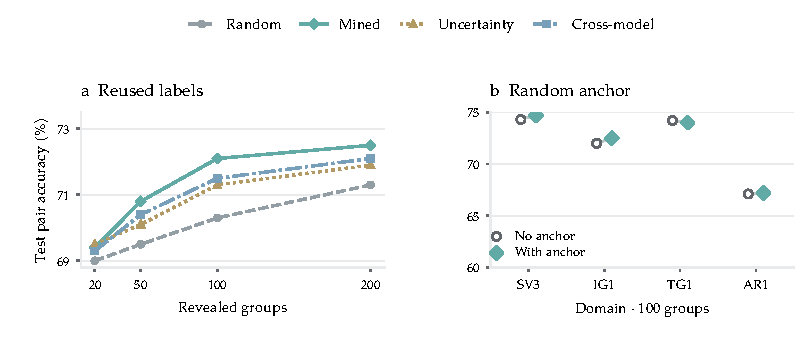
\includegraphics[width=5.4in]{figures/ideal_scenario/mining.pdf}

\caption{\textbf{Preference-mining efficiency.}
(a) Held-out pair accuracy versus revealed groups in existing-label replay.
(b) Mined feedback with and without the random anchor at the same 100-group budget, by domain.}
\label{fig:acquisition}
\end{figure}

\begin{table}[!htbp]
\caption{\textbf{Mining and end-to-end comparison.}
The two-by-two design uses 100 revealed groups in every cell.
Decisive-pair accuracy is in percent.
Total model-and-tool cost includes mining and search in relative units, not human labor.
The two search policies are fixed patience and EvalOpt.}
\label{tab:mining-results}
\centering\small
\begin{tabularx}{\linewidth}{@{}YYcc@{}}
\toprule
Feedback & Search & Pair acc. & Total cost\\
\midrule
% SIMULATED IDEAL SCENARIO; not experimental results.
Random & Fixed patience & 67.0 & 102\\
Mined & Fixed patience & 68.2 & 106\\
Random & EvalOpt & 70.3 & 102\\
Mined & EvalOpt & 72.1 & 106\\

\bottomrule
\end{tabularx}
\end{table}
\paragraph{What disagreement mining selects.}
We examine SV3, IG1, TG1, and AR1 at the same 100-group feedback budget, combining 80 ranked pairs and 20 random-anchor pairs into the selected feedback set.
Each domain has 224 eligible Train groups with decisive overall preference labels, one pair per group, and five selection seeds.
Existing labels retain their source semantics; source ties and missing labels are outside this diagnostic cohort.
This composition diagnostic uses a separate two-rubric-source configuration, not the four-judge experimental roster.
Both sources cover four dimensions and overall quality, supplemented by browser requirement checks (SV3), CIDEr (IG1), or SummaC (TG1); AR1 has no additional checker.
For each dimension, comparison coverage is the fraction of pairs with at least two available source-group votes, including tied votes.
Across the four dimensions, its ranges for Pool / Selected are % SIMULATED_LAYOUT_SCENARIO; not observed human/model judgments.
SV3 95.1--100.0\% / 95.6--100.0\%; IG1 94.6--100.0\% / 95.2--100.0\%; TG1 94.6--99.6\% / 95.6--99.0\%; AR1 93.8--98.7\% / 95.2--98.6\%.

Missing votes remain unavailable rather than counting as agreement.

% Keep this half-page diagnostic with text rather than on a float-only page.
\begin{figure}[!htb]
\centering
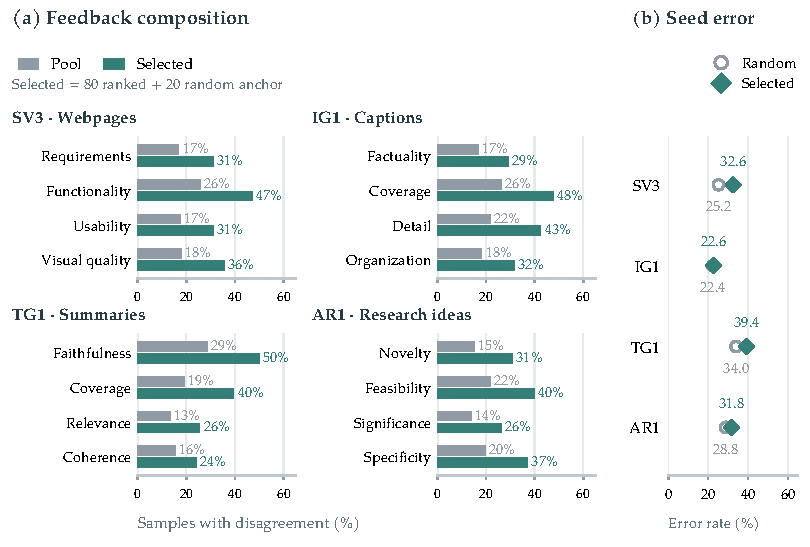
\includegraphics[width=5.4in]{figures/mining_diagnostics/mining_diagnostics.pdf}
\caption{\textbf{Feedback composition and Seed errors.}
(a) Pairs with observed evaluator disagreement on each dimension, as a percentage of all pairs in the Pool (gray) or Selected feedback (teal).
Selected combines 80 ranked and 20 random-anchor pairs. A pair can contribute to several dimensions, so percentages need not sum to 100\%.
(b) Seed error for Selected versus 100 uniformly sampled pairs, using decisive overall labels and counting evaluator score ties as errors.
Pool percentages use 224 pairs; Selected and Random percentages pool 500 appearances across five selections, not independent samples.}
\label{fig:mining-diagnostics}
\end{figure}

Figure~\ref{fig:mining-diagnostics}a describes selection's effect on observed disagreements, which depend on the evaluators and their coverage rather than intrinsic dimension difficulty.
Panel~b audits Seed errors using overall preference labels revealed only after selection, without dimensional human labels.
Learning benefit is assessed separately in Figure~\ref{fig:acquisition}.

For the anchor audit, we deduplicate pairs across selection seeds and retain those with decisive human preferences and matching non-tied overall votes from both rubric judges.
The counts opposing this shared model preference are % SIMULATED_LAYOUT_SCENARIO; not observed human/model judgments.
SV3 4/55, IG1 5/59, TG1 5/51, AR1 4/47.

These conditional counts describe shared errors accessible to random sampling; the fixed-budget anchor comparison tests their contribution to learning.

\subsection{Additional human annotation experiment}
\label{app:slide-pilot}
This separate SV1 study tests whether selecting annotation questions yields useful feedback for evaluator revision.
SV1's C1 comparison uses our own human annotations; the sampling study below separately evaluates how to allocate additional annotation questions, rather than assuming a public slide-preference release.
For collection, we plan to use briefs from \href{https://huggingface.co/datasets/tyrionhuu/PPTBench-Generation}{PPTBench-Generation}, with two single-slide outputs per brief generated by GPT-5.6 Sol under a shared prompt and budget with different generation seeds.
The public resource supplies inputs, not the pairwise human labels for this study.
The design allocates 200 Train, 40 Val, and 120 Test brief groups, independently of C1 and the four-domain analyses.
Source-document and near-duplicate groups must remain within one split, and the source manifest, generation settings, renderer, and output hashes must be frozen before mining.
Eligibility requires a self-contained brief, accessible supporting material, and two inspectable renders; exclusions precede both sampling arms.

\paragraph{Question selection and blinding.}
The mined arm selects eight random-anchor pairs before ranking and 32 pairs by the within-dimension disagreement count in Equation~\ref{eq:conflict}.
For each ranked pair, it samples one or two conflicting dimensions and one or two additional non-conflicting dimensions, uniformly without replacement within each set.
The requested counts are chosen by independent input hashes before annotation and capped by the available dimensions in each set.
Anchor pairs receive three uniformly sampled dimensions.
Every selected pair also receives an overall question.
The random arm samples 40 pairs uniformly from the same Train pool and matches the mined arm's per-pair question-count distribution, but samples dimensional questions uniformly.
The criteria in Table~\ref{tab:data-sources} form a question bank, not a mandatory checklist: the interface displays only the sampled questions, with no fields for unqueried dimensions.
% SIMULATED layout scenario; source: data/slide_pilot_preview.json
Each arm requests 157 questions (10 pairs with 3, 23 pairs with 4, 7 pairs with 5 questions), yielding 314 initial individual ratings.

The comparison tests the combined pair-and-dimension sampling policy.

Raters see the brief, supporting material, and equally sized slide renders in randomized A/B positions, with model identities, signal votes, and sampling status hidden.
Two independent raters answer overall preference first, followed by the sampled dimensional questions in randomized order.
Each question offers A, B, tie, or unable to judge; tie means comparable quality, whereas inability indicates insufficient evidence.
Raters must be fluent in the brief's language and familiar with presentation review, with rubric calibration on separate practice items before annotation.
An identical non-missing response from both raters is accepted, including a tie.
Otherwise, a third blinded rater answers that question, and two matching non-missing responses determine its label; without that agreement it remains unresolved.
Unasked dimensions remain absent rather than being filled by overall preference or model votes.

\paragraph{Annotation efficiency.}
A usable label is a resolved preference or tie.
Before acquisition, the pilot Seed records pointwise scores for each slide on the question-bank criteria and overall quality.
These frozen scores are compared with decisive human labels separately for dimensional and overall judgments; a Seed score tie counts as an error.
Table~\ref{tab:slide-pilot}a reports both usable labels and discovered Seed errors per 100 individual ratings, including third-rater adjudication.
The two arms have the same initial budget, not necessarily the same realized adjudication cost or annotation time.
Shared pair--question labels are reused across arms, while each arm is charged the ratings needed to obtain its own feedback set.
Val and Test annotation costs are common to both arms and reported separately from Train acquisition.

\begin{table}[!htbp]
\caption{\textbf{Slide annotation and feedback use.}
(a) Acquisition cost and feedback yield for random and mined questions. Agreement uses questions both initial raters can judge; efficiency includes adjudication ratings.
(b) Test accuracy of Val-retained checkpoints, with mean $\pm$ sample standard deviation across five searches using each fixed feedback set.}
\label{tab:slide-pilot}
\centering\small
\begin{tabularx}{\linewidth}{@{}Yrr@{}}
\toprule
\multicolumn{3}{@{}l}{(a) Annotation cost and feedback yield}\\
Measure & Random & Mined\\
\midrule
% SIMULATED layout scenario; source: data/slide_pilot_preview.json
Pairs / requested questions & 40 / 157 & 40 / 157 \\
Initial + adjudication ratings & 314 + 45 & 314 + 54 \\
Usable labels / questions & 153/157 (97.5\%) & 144/157 (91.7\%) \\
Final ties / unresolved & 4 / 4 & 4 / 13 \\
Initial unable ratings & 11 & 8 \\
Initial exact agreement & 112/146 (76.7\%) & 103/149 (69.1\%) \\
Overall Seed errors / decisive labels & 8/36 & 7/32 \\
Dimension Seed errors / decisive labels & 28/113 & 29/108 \\
Usable labels per 100 ratings & 42.6 & 39.1 \\
Overall Seed errors per 100 ratings & 2.23 & 1.90 \\
Dimension Seed errors per 100 ratings & 7.80 & 7.88 \\

\bottomrule
\end{tabularx}
\smallskip
\begin{tabularx}{\linewidth}{@{}Yrrr@{}}
\toprule
\multicolumn{4}{@{}l}{(b) Feedback used by the same evolution policy}\\
Evaluator & Test accuracy & Gain over Seed & Gain over random\\
\midrule
% SIMULATED layout scenario; source: data/slide_pilot_preview.json
Seed & 79.6\% & -- & -- \\
EvalOpt + random & $83.3 \pm 2.7$\% & +3.7 pp & -- \\
EvalOpt + mined & $83.5 \pm 1.9$\% & +3.9 pp & +0.2 pp \\

\bottomrule
\end{tabularx}
\end{table}

\paragraph{Evolution and assessment.}
Both arms start from the same Seed and EvalOpt policy, with caps of 100,000 model tokens and 100 tool calls per search, including diagnostics and Val access.
Pool scoring is accounted for separately rather than attributed to human labor.
Only the acquired Train labels are exposed to revision, preserving their dimension identities, ties, and missing fields.
Five paired search seeds per arm use these fixed feedback sets and the same Val schedule.
The three scheduled Val comparisons retain a checkpoint only on a strict accuracy improvement, with ties retaining the earlier checkpoint.
Test is read only after checkpoint selection and never reranks candidates.
Three blinded raters judge overall preference for every Val and Test pair, requiring two matching non-missing responses under the same rule as Train.
% SIMULATED layout scenario; source: data/slide_pilot_preview.json
The frozen Test cohort contains 108 decisive pairs, 0 ties, and 12 unresolved pairs out of 120; accuracy uses the decisive subset.
Val contains 38 decisive pairs, 1 tie, and 1 unresolved pair out of 40.

These held-out annotations require 120 Val and 360 Test ratings shared by both arms.
Table~\ref{tab:slide-pilot}b reports all five retained outcomes, not the best search, and their variation is conditional on one acquisition per arm rather than five independent annotation studies.
The efficiency and accuracy comparisons answer different questions: more disagreement does not guarantee more usable feedback or a better retained evaluator.

\section{Downstream applications}
\label{app:downstream}
\subsection{Shared setup and assessment}
\label{app:downstream-assessment}
C2 tests critique-guided refinement and C3 tests reward-guided training, using the shared assessment in Table~\ref{tab:readiness} for Figure~\ref{fig:budget-tests}b.
\begin{table}[!htbp]
\caption{\textbf{Downstream assessment by domain.} Human preference is the primary endpoint in C2/C3. Computable measures assess specific attributes, not a shared cross-domain quality score.}
\label{tab:readiness}
\centering\small
\begin{tabularx}{\linewidth}{@{}P{1.45cm}YYY@{}}
\toprule
ID / inputs & Human rubric source & Human assessment & Computable complement\\
\midrule
SV3 / WebDev & Adapted WebGen-Bench appearance criteria and operation--expected-result checks \citep{lu2025webgen} & Requirement satisfaction, usability and appearance; pairwise overall choice & Render success; reserved requirement-test pass rate\\
IG1 / DOCCI & CapArena annotation guidelines, Appendix H \citep{cheng2025caparena} & Precision, salient information, hallucination and conciseness; pairwise choice & SPICE precision, recall and F1 against the DOCCI description\\
TG1 / TL;DR & TL;DR comparison and rating instructions, Appendix C.5 \citep{stiennon2020summarize} & Overall choice; 1--7 coherence, accuracy, coverage and overall ratings & ROUGE-L F1 against the human TL;DR; SummaCConv as an optimization-exposed diagnostic\\
AR1 / Ideation Arena & Human-review criteria, Appendix A.2 \citep{chen2026ideation} & Overall choice; novelty, feasibility, significance and specificity preferences & None\\
\bottomrule
\end{tabularx}
\end{table}
\paragraph{Data allocation.}
Each domain uses 512 training, 64 development, and 200 final-assessment inputs, disjoint from evaluator Train/Val/Test and the timed-annotation pool.
Freeze all roles before mining, without later additions.
C2/C3 share final-assessment inputs but obtain separate outputs and new judgments, requiring 1,296 eligible groups per domain: 520 for C1 and 776 downstream, counted once across arms and seeds.
Development inputs support generator checks and reward calibration, not evaluator evolution.
Evaluator-search seeds 11/22/33 are paired with generator or training seeds in prespecified blocks, not selected by evaluator score.

\paragraph{Source overlap and eligibility.}
WebDev groups use normalized user specifications, with repeated requests and near-duplicate templates kept together; restrict the cohort to single-turn tasks with executable artifacts.
CapArena's human comparisons reuse DOCCI images, so image IDs and near-duplicate scenes are grouped jointly across both releases.
Use CapArena for C1, DOCCI Train for downstream training/development, and DOCCI Test images outside CapArena for downstream assessment; reference descriptions are withheld from generators.
TL;DR groups use post IDs and normalized post text; downstream inputs come from the released source-and-reference corpus after removing all comparison-cohort posts.
For ideation, group identical and near-duplicate literature contexts, using the same seed-paper group wherever its identity is available.
Shared background citations alone do not merge otherwise distinct contexts; quantify this overlap and record unavailable seed identities in the manifest.
The complete supplied literature context must fit both the generator and reward evaluator; exclude overlength inputs before allocation rather than truncating evidence underlying an existing preference label.
Public-source counts precede these eligibility checks, and API processing also requires permission under each source's terms.

\begin{table}[!htbp]
\caption{\textbf{Domain-specific downstream inputs and generation limits.}
C2 uses GPT-5.6 Sol; C3 uses Qwen3.5-9B. $L$ is the output token cap. Shared allocations and study-specific settings are given in the text.}
\label{tab:downstream-config}
\centering\small
\begin{tabularx}{\linewidth}{@{}lYrr@{}}
\toprule
Domain & Input source & Input token cap & $L$\\
\midrule
SV3 & WebDev Arena & 16,384 & 4,096\\
IG1 & DOCCI & 8,192 & 512\\
TG1 & TL;DR & 8,192 & 256\\
AR1 & Ideation Arena & 32,768 & 1,536\\
\bottomrule
\end{tabularx}
\end{table}

\paragraph{Models and inputs.}
Table~\ref{tab:downstream-config} specifies domain-specific limits.
GPT-5.6 Sol generates C2 initial outputs and revisions, with reasoning effort \texttt{none} and no temperature or top-$p$ override.
C3 uses the public post-trained \href{https://huggingface.co/Qwen/Qwen3.5-9B}{Qwen3.5-9B} checkpoint, revision \texttt{c20223623576}, in all four domains, with thinking disabled throughout training and assessment.
The Base, Seed-reward, and EvalOpt-reward arms share this checkpoint and tokenizer; only the two reward arms receive policy updates.
Seed and EvalOpt critiques and rewards use the GPT-5.6 Sol evaluator settings in Table~\ref{tab:run-config}.
The captioner receives the image, but not the DOCCI reference.
The webpage model generates a complete HTML/CSS/JavaScript artifact; browser execution supplies evaluator evidence rather than an extra trainable policy.
Summarization uses the source post, and ideation uses a closed literature context with no online retrieval.

\paragraph{Human assessment.}
Three blinded raters assess each output pair under fixed, shared instructions after calibration on disjoint examples.
They see the task, permitted evidence, and anonymized outputs, without critiques, rewards, automatic scores, or reference captions/summaries.
Choices are A, B, tie, or unable to judge; AR1 also records Both Bad, counted as a tie and reported separately.
AR1 raters must know the topic and supplied literature, deferring unsupported judgments.
Tie-aware preference is $(W+T/2)/(W+L+T)$, with abstentions and missing outputs reported separately.
Record rater backgrounds, calibration, agreement, and person-time.

Table~\ref{tab:readiness} gives domain criteria and rubric sources.
SV3 requires inspecting the running page, including interactions, with task-specific operation--expected-result checks.
Its 1--5 appearance anchors adapt WebGen-Bench's model-grading prompt rather than an existing human pairwise instrument.
IG1 follows CapArena's human guidelines, including not rewarding length alone; TG1 uses TL;DR's comparison instructions and separate 1--7 rating anchors.
AR1 asks which proposal merits investment under the listed criteria, assessing a proposal rather than a completed finding \citep{si2025ideas}.

\paragraph{Regression judgments.}
Each regression flag identifies a newly introduced material problem relative to the reference output: broken required interaction or unusable layout (SV3), a salient hallucination or lost essential description (IG1), a central factual distortion or omission (TG1), or an unsupported central premise or infeasible experimental dependency (AR1).
Raters identify the affected requirement, image region, source passage, or proposal statement.
Majority vote determines the flag; minor stylistic changes do not qualify.
Regression is measured against $y_0$ in C2 and Base in C3, not necessarily the pairwise comparison arm.

\paragraph{Executable and reference-based measures.}
SV3 runs prespecified assertions in isolated Chromium at $1280\!\times\!800$ with a 30-second load limit.
Render success requires nonblank task content; requirement pass rate averages the fraction of passed assertions equally over tasks.
Artifact-caused failures fail dependent assertions, while browser-service outages remain missing.
IG1 uses the released SPICE parser \citep{anderson2016spice} on complete captions and matching DOCCI references, reporting tuple precision, recall, and F1.
Reference omissions and parser errors limit SPICE, with hallucination assessed separately by humans.
TG1 references are human summaries matched by post ID before cohort freezing, not model outputs or preferred comparison candidates.
ROUGE-L F1 \citep{lin2004rouge} uses \texttt{rouge-score}, English stemming, and no truncation.
SummaCConv \citep{laban2022summac} uses the released \texttt{vitc} sentence-level model and mean aggregation.
Because it also participates in mining, SummaC is an optimization-exposed diagnostic, not an independent endpoint, and its news training limits interpretation on Reddit posts.

\paragraph{Assessment boundary and reporting.}
Reserve SPICE, ROUGE-L, final reference texts, and browser assertions from mining, evaluator tools, critique, reward, and checkpoint selection, while allowing general browser execution.
Table~\ref{tab:data-sources} surveys alternatives, not the executed tool roster.
Assess the same final outputs from every arm, recording versions, preprocessing, manifests, output lengths, completion counts, and missing outcomes.
Report per-domain means and paired differences with the uncertainty protocol in Appendix~\ref{app:measurement}, without averaging incompatible metric scales.
Table~\ref{tab:downstream-detail} summarizes preference and per-arm outcomes.

\subsection{Critique-guided refinement}
C2 branches each fresh initial output $y_0$ into no-critic, Seed-critic, and EvalOpt-critic arms, each with two successive revisions.
Arms share the generator, settings, task evidence, and output cap $L$; critic arms additionally receive a frozen evaluator's critique, capped at 512 tokens per round under a common format.
The current output and task are available in every round, including the same captioning image.
Each branch generates at most $3L$ tokens including $y_0$, with critique and tool costs charged separately.
No intermediate human judgments or best-of-$N$ selection are available.
Seeds identify paired data/output blocks rather than deterministic API samples.

The primary comparison is EvalOpt versus Seed critique; secondary comparisons are EvalOpt versus no critic and each revised arm versus $y_0$.
Five comparisons over 200 inputs, three seeds, and three raters allocate 9,000 pair judgments per domain, excluding adjudication and separate attribute ratings.

\begin{table}[!htbp]
\caption{\textbf{Downstream controls and per-arm outcomes.}
Preference, major regression, and invalidity are percentages.
Merged risk cells describe the first arm relative to $y_0$ (C2) or Base (C3), independently of the comparator.
Values equally weight the four domains.}
\label{tab:downstream-detail}
\centering\small
\begin{tabularx}{\linewidth}{@{}Yccc@{}}
\toprule
Contrast & Pref. & Major regression & Invalid\\
\midrule
% SIMULATED IDEAL SCENARIO; not experimental results.
C2: Seed / $y_0$ & 252/48/180 & 57.5 & 10.0 & 1.0 & 480/480\\
C2: IterEval / $y_0$ & 302/52/126 & 68.3 & 4.8 & 0.6 & 480/480\\
C2: IterEval / Seed & 270/48/162 & 61.3 & 4.8 & 0.6 & 480/480\\
C2: IterEval / no critic & 294/42/144 & 65.6 & 4.8 & 0.6 & 480/480\\
C3: Seed / Base & 80/24/56 & 57.5 & 12.5 & 1.3 & 160/160\\
C3: IterEval / Base & 96/24/40 & 67.5 & 7.5 & 0.6 & 160/160\\
C3: IterEval / Seed & 90/20/50 & 62.5 & 7.5 & 0.6 & 160/160\\

\bottomrule
\end{tabularx}
\end{table}
\subsection{Reward-guided training}
\label{app:training}
C3 compares policies trained with frozen Seed or EvalOpt rewards against an untrained Base.
Reward arms share the Base checkpoint, LoRA/GRPO settings, inputs, tools, and update budget; only the frozen evaluator differs.
Both rewards score a common starting-policy pool for variance, ties, validity, and sensitivity to length or unsupported detail, under development-frozen preflight thresholds and stopping rules.

Only the preflight pool is shared: once policies diverge, each samples its own online trajectories.
\paragraph{Training recipe.}
Each reward arm starts from the same policy checkpoint with LoRA rank 16, scale 32, and dropout 0.05 on the language model's attention, gated-delta, and MLP projection layers.
Embeddings, the vision encoder, and the vision--language merger remain frozen; exact adapter target names are fixed in the run manifest.
GRPO uses eight distinct prompts per update and four on-policy completions per prompt, giving 32 sequences per optimizer update.
Two seeded shuffled passes over the 512 training inputs give 128 updates and 4,096 completions per arm and seed.
Generation uses temperature 0.8 and top-$p$ 0.95, with the task-specific caps in Table~\ref{tab:downstream-config}.
Use AdamW with learning rate $10^{-5}$, $(\beta_1,\beta_2)=(0.9,0.95)$, weight decay 0.01, and gradient-norm clipping at 1.0.
The first 13 updates warm up linearly, followed by cosine decay to $10^{-6}$.
The clipped policy objective uses threshold 0.2, a fixed KL coefficient 0.02 against Base, and one optimization pass over each rollout batch.
Advantages are standardized within each four-completion group with denominator floor $10^{-6}$; zero-variance groups are retained in accounting but contribute zero policy-gradient advantage.

\paragraph{Reward and final assessment.}
Each frozen evaluator scores the same 256 Base completions (four per development input) to set its reward mean and standard deviation.
Standardize scores with these fixed calibration moments and clip to $[-3,3]$, assigning invalid artifacts $-3$; use no additional correctness or length reward.
One evaluator execution supplies each training reward, with the same decoding and tool limits in both arms.
Required scorer failures interrupt the run rather than becoming fabricated rewards.
Score ties, zero-variance groups, invalid outputs, and truncation rates are retained as diagnostics.
Assess the terminal step-128 checkpoint; earlier training checkpoints are diagnostic only and are not selected by Test performance.
Final generation uses temperature 0.7 and top-$p$ 0.9 with one output per input and seed.
Independent assessment compares EvalOpt-reward with Seed-reward and both with Base, allocating 5,400 pair judgments per domain across 200 inputs, three seeds, and three raters.
Reward increases alone do not establish quality gains.
The full training allocation is 24 runs (four domains, two reward arms, three seeds), with a 48-hour wall-clock ceiling per run; interruptions remain visible and are not silently replaced by successful seeds.
\FloatBarrier
